\documentclass[preview]{standalone}
\usepackage{caption}
\usepackage{tikz}
\usetikzlibrary{fit, arrows}
\captionsetup[figure]{labelformat=empty}

\begin{document}
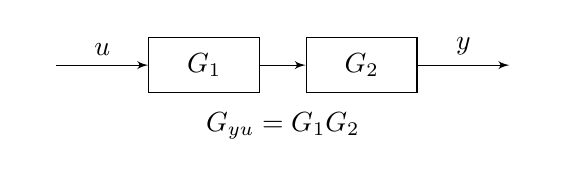
\begin{tikzpicture}[auto, node distance=2cm,>=latex']
  \tikzstyle{block} = [draw, rectangle, minimum height=2em, minimum width=4em]
  \node (input) {};
  \node [block, right of=input] (G1) {$G_1$};
  \node [block, right of=G1] (G2) {$G_2$};
  \node [right of=G2] (output) {};
  \node [fit=(input) (G1) (G2) (output), label=below:{$G_{yu}=G_1G_2$}] {};

  \draw [->] (input) -- node {$u$} (G1);
  \draw [->] (G1) -- node {} (G2);
  \draw [->] (G2) -- node {$y$} (output);
\end{tikzpicture}
\end{document}
